\documentclass[border=10pt]{standalone}
\usepackage[T1]{fontenc}
\usepackage[default]{sourcesanspro}
\usepackage{tikz}
\usepackage{xcolor}
\usetikzlibrary{positioning,calc}

\begin{document}
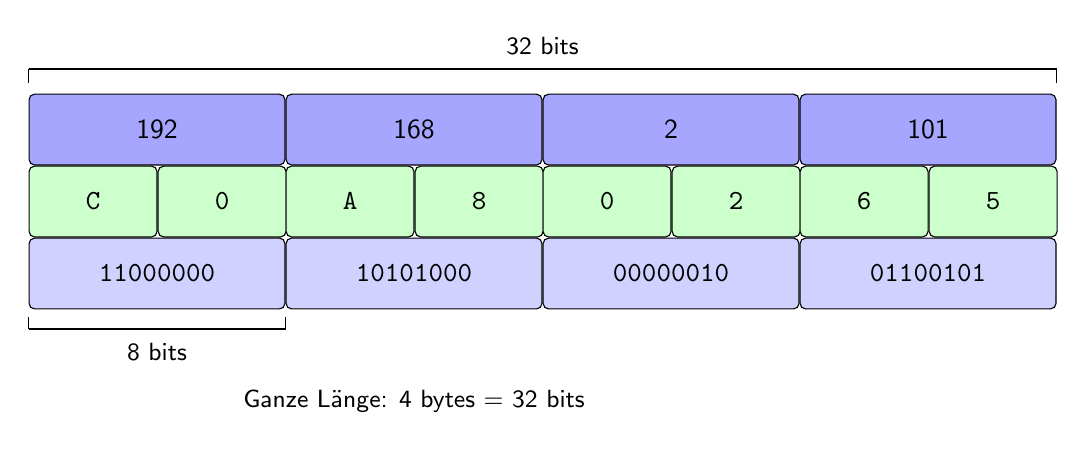
\begin{tikzpicture}[
  font=\sffamily,
  oct/.style={
    draw,
    rounded corners=2pt,
    minimum width=3.25cm,
    minimum height=9mm,
    align=center
  },
  dec/.style={oct, fill=blue!35},     % darker pastel blue
  bin/.style={oct, fill=blue!18},     % lighter pastel blue
  note/.style={font=\sffamily\small},
  brace/.style={line width=0.6pt},
  hex/.style={
    draw,
    rounded corners=2pt,
    minimum width=1.625cm,           % half of oct width -> two boxes per byte
    minimum height=9mm,
    align=center,
    fill=green!20                    % light pastel green
  }
]

% --- Row 1: decimal octets ---
\node[dec] (d1) {192};
\node[dec, right=0pt of d1] (d2) {168};
\node[dec, right=0pt of d2] (d3) {2};
\node[dec, right=0pt of d3] (d4) {101};

% --- Row 2: hex octets split into nibbles (2 boxes per byte) ---
\def\halfhex{0.8125cm}

% Byte 1: C0
\node[hex, below=0pt of d1, xshift=-\halfhex] (h1a) {\ttfamily C};
\node[hex, right=0pt of h1a] (h1b) {\ttfamily 0};

% Byte 2: A8
\node[hex, below=0pt of d2, xshift=-\halfhex] (h2a) {\ttfamily A};
\node[hex, right=0pt of h2a] (h2b) {\ttfamily 8};

% Byte 3: 02
\node[hex, below=0pt of d3, xshift=-\halfhex] (h3a) {\ttfamily 0};
\node[hex, right=0pt of h3a] (h3b) {\ttfamily 2};

% Byte 4: 65
\node[hex, below=0pt of d4, xshift=-\halfhex] (h4a) {\ttfamily 6};
\node[hex, right=0pt of h4a] (h4b) {\ttfamily 5};

% --- Row 3: binary octets ---
\node[bin, below=0pt of h1a, xshift=\halfhex] (b1) {\ttfamily 11000000};
\node[bin, below=0pt of h2a, xshift=\halfhex] (b2) {\ttfamily 10101000};
\node[bin, below=0pt of h3a, xshift=\halfhex] (b3) {\ttfamily 00000010};
\node[bin, below=0pt of h4a, xshift=\halfhex] (b4) {\ttfamily 01100101};

% --- Bit-length "bars" ---
% 8-bit bar below the first binary octet
\draw[brace] ($(b1.south west)-(0,2.5mm)$) -- ($(b1.south east)-(0,2.5mm)$);
\draw[brace] ($(b1.south west)-(0,2.5mm)$) -- ($(b1.south west)-(0,1.0mm)$);
\draw[brace] ($(b1.south east)-(0,2.5mm)$) -- ($(b1.south east)-(0,1.0mm)$);
\node[note, below=3.1mm of b1.south] {8 bits};

% 32-bit bar above the entire decimal row
\coordinate (L) at ($(d1.north west)+(0,3.1mm)$);
\coordinate (R) at ($(d4.north east)+(0,3.1mm)$);
\draw[brace] (L) -- (R);
\draw[brace] (L) -- ($(L)+(0,-1.8mm)$);
\draw[brace] (R) -- ($(R)+(0,-1.8mm)$);
\node[note] at ($(L)!0.5!(R)+(0,3mm)$) {32 bits};

% --- Total length label centered under everything ---
\node[note, below=9mm of b2] {Ganze L\"ange: 4 bytes = 32 bits};

\end{tikzpicture}
\end{document}
